\ylDisplay{Sfäärilised peeglid} % Ülesande nimi
{Tundmatu autor} % Autor
{lõppvoor} % Voor
{2016} % Aasta
{P 10} % Ülesande nr.
{3} % Raskustase
{
% Teema: Valgusõpetus
\ifStatement
Joonisel on kujutatud kahe sfäärilise peegli optilised peateljed ja valguspunkti $A$ ja selle kujutise $A'$ asukohad kummagi peegli jaoks eraldi. Konstrueerige kummagi peegli pinna lõikepunkt optilise peateljega ja peeglite optilised keskpunktid.
\begin{center}
	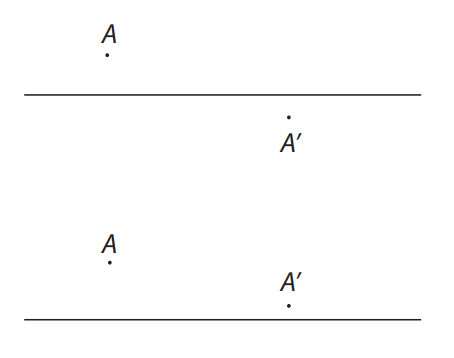
\includegraphics[width=0.5\linewidth]{2016-v3p-10-yl.PNG}
\end{center}
\fi
\ifHint
Konstrueerimsiel lähtu peegeldumise seadustest.
\fi
\ifSolution
Konstrueerime kujutise punktiga sümmeetrilise punkti teisel pool optilist telge. Valguspunktist tulnud kiir läbib seda punkti ja peegeldudes peegli lagipunktilt läbib kujutise punkti. Teiseks kiireks on kiir, mis läbib eseme, kujutise ja peegli optilise keskpunkti ning peegeldub peeglilt sama teed tagasi.
\begin{center}
	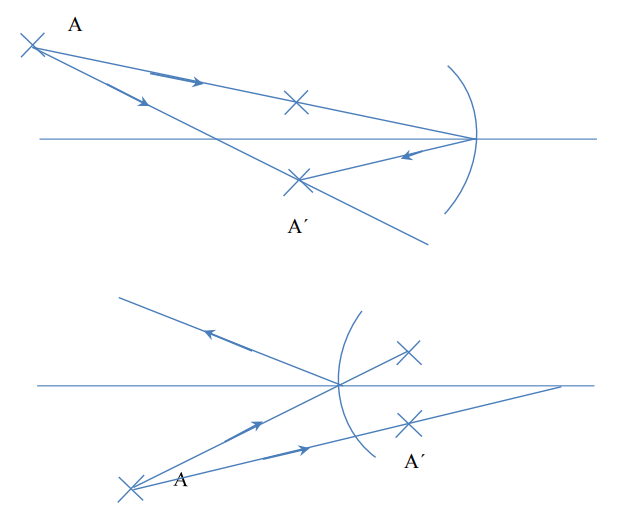
\includegraphics[width=0.5\linewidth]{2016-v3p-10-lah.PNG}
\end{center}
\fi
}
